\pagenumbering{gobble}  % Pas de numérotation
\begin{titlepage}
    \vspace*{-10px}
    
\includegraphics[height=80px]{Images/logo_phelma.pdf}
    \vspace*{-80px}
\begin{flushright}
    \vspace*{-10px}
    
\includegraphics[height=80px]{Images/Logo_Neel.pdf}
\end{flushright}

\vspace*{1.5cm}
\begin{center}
\rule{\linewidth}{0.5mm}\\[0.4cm]
{\huge{\bfseries Rapport de Projet de Fin d'Études}\\[0.4cm]
Caractérisation de pointes fibrées pour nano-pinces optiques et plasmoniques\\[0.4cm]}
\rule{\linewidth}{0.5mm}\\[0.5cm]

\LARGE{\textsc{Félix Piédallu}}\\[0.7cm]
\large{\textsc{Filière PNS 2015-2016}}\\[2cm]

\Large{Au sein de l'équipe Nano-Optique et Forces}\\[1cm]

\Large{Sous la direction de Jochen \textsc{Fick}}\\[2cm]

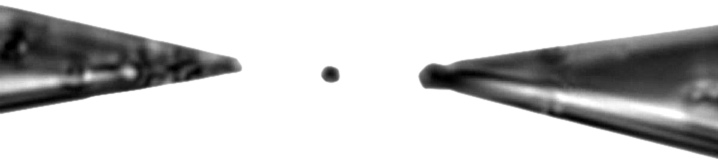
\includegraphics[width=\textwidth]{Images/Illustration.png}\\[1cm]


\end{center}
\end{titlepage}

\tableofcontents        % Table des matières avec liens, générée automatiquement.
\newpage
\listoffigures
\pagenumbering{arabic}  % Numérotation de retour !
